\documentclass{standalone}
\usepackage{tikz}
\usetikzlibrary{patterns, positioning}


\begin{document}
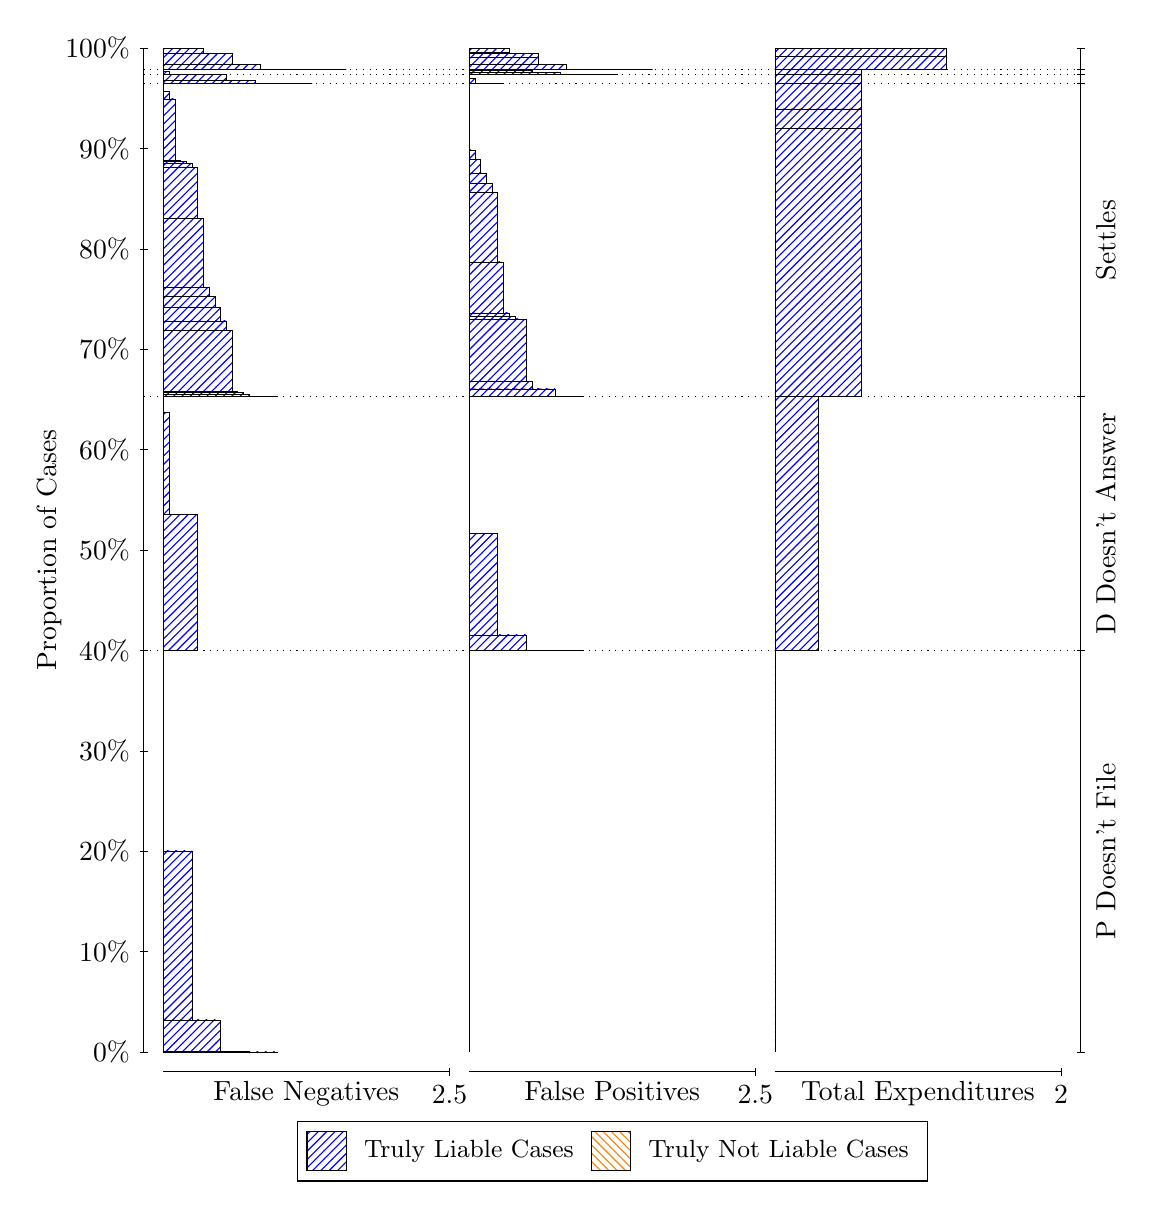
\begin{tikzpicture}
\draw[black, very thin] (1.5,1.75) -- (1.5,14.5);
\node[rotate=90, text=black, anchor=center] at (0.3, 8.125) {Proportion of Cases};
\draw[black, very thin] (1.45,1.75) -- (1.55,1.75);
\node[text=black, anchor=east] at (1.45, 1.75) {0\%};
\draw[black, very thin] (1.45,3.025) -- (1.55,3.025);
\node[text=black, anchor=east] at (1.45, 3.025) {10\%};
\draw[black, very thin] (1.45,4.3) -- (1.55,4.3);
\node[text=black, anchor=east] at (1.45, 4.3) {20\%};
\draw[black, very thin] (1.45,5.575) -- (1.55,5.575);
\node[text=black, anchor=east] at (1.45, 5.575) {30\%};
\draw[black, very thin] (1.45,6.85) -- (1.55,6.85);
\node[text=black, anchor=east] at (1.45, 6.85) {40\%};
\draw[black, very thin] (1.45,8.125) -- (1.55,8.125);
\node[text=black, anchor=east] at (1.45, 8.125) {50\%};
\draw[black, very thin] (1.45,9.4) -- (1.55,9.4);
\node[text=black, anchor=east] at (1.45, 9.4) {60\%};
\draw[black, very thin] (1.45,10.675) -- (1.55,10.675);
\node[text=black, anchor=east] at (1.45, 10.675) {70\%};
\draw[black, very thin] (1.45,11.95) -- (1.55,11.95);
\node[text=black, anchor=east] at (1.45, 11.95) {80\%};
\draw[black, very thin] (1.45,13.225) -- (1.55,13.225);
\node[text=black, anchor=east] at (1.45, 13.225) {90\%};
\draw[black, very thin] (1.45,14.5) -- (1.55,14.5);
\node[text=black, anchor=east] at (1.45, 14.5) {100\%};

\draw[black, very thin] (13.4,1.75) -- (13.4,14.5);
\draw[black, very thin] (13.35,1.75) -- (13.45,1.75);
\node[anchor=west] at (13.35, 1.75) {};
\draw[black, very thin] (13.35,6.8489) -- (13.45,6.8489);
\node[anchor=west] at (13.35, 6.8489) {};
\draw[black, very thin] (13.35,10.072) -- (13.45,10.072);
\node[anchor=west] at (13.35, 10.072) {};
\draw[black, very thin] (13.35,14.052) -- (13.45,14.052);
\node[anchor=west] at (13.35, 14.052) {};
\draw[black, very thin] (13.35,14.163) -- (13.45,14.163);
\node[anchor=west] at (13.35, 14.163) {};
\draw[black, very thin] (13.35,14.224) -- (13.45,14.224);
\node[anchor=west] at (13.35, 14.224) {};
\draw[black, very thin] (13.35,14.5) -- (13.45,14.5);
\node[anchor=west] at (13.35, 14.5) {};

\draw[black, very thin, pattern color=blue, pattern=north east lines] (1.75,1.75) rectangle (3.2033,1.75);
\draw[black, very thin, pattern color=blue, pattern=north east lines] (1.75,1.75) rectangle (2.84,1.7534);
\draw[black, very thin, pattern color=blue, pattern=north east lines] (1.75,1.7534) rectangle (2.4767,2.158);
\draw[black, very thin, pattern color=blue, pattern=north east lines] (1.75,2.158) rectangle (2.1133,4.3029);
\draw[black, very thin, pattern color=orange, pattern=north west lines] (1.75,4.3029) rectangle (1.75,4.3029);
\draw[black, very thin, pattern color=blue, pattern=north east lines] (1.75,4.3029) rectangle (1.75,6.8489);
\draw[black, very thin, pattern color=blue, pattern=north east lines] (1.75,6.8489) rectangle (2.186,8.5806);
\draw[black, very thin, pattern color=blue, pattern=north east lines] (1.75,8.5806) rectangle (1.8227,9.8734);
\draw[black, very thin, pattern color=orange, pattern=north west lines] (1.75,9.8734) rectangle (1.75,9.8734);
\draw[black, very thin, pattern color=blue, pattern=north east lines] (1.75,9.8734) rectangle (1.75,10.072);
\draw[black, very thin, pattern color=blue, pattern=north east lines] (1.75,10.072) rectangle (3.2033,10.072);
\draw[black, very thin, pattern color=blue, pattern=north east lines] (1.75,10.072) rectangle (3.058,10.072);
\draw[black, very thin, pattern color=blue, pattern=north east lines] (1.75,10.072) rectangle (2.9127,10.072);
\draw[black, very thin, pattern color=blue, pattern=north east lines] (1.75,10.072) rectangle (2.84,10.097);
\draw[black, very thin, pattern color=blue, pattern=north east lines] (1.75,10.097) rectangle (2.7673,10.128);
\draw[black, very thin, pattern color=blue, pattern=north east lines] (1.75,10.128) rectangle (2.6947,10.135);
\draw[black, very thin, pattern color=blue, pattern=north east lines] (1.75,10.135) rectangle (2.622,10.919);
\draw[black, very thin, pattern color=blue, pattern=north east lines] (1.75,10.919) rectangle (2.5493,11.035);
\draw[black, very thin, pattern color=blue, pattern=north east lines] (1.75,11.035) rectangle (2.4767,11.21);
\draw[black, very thin, pattern color=blue, pattern=north east lines] (1.75,11.21) rectangle (2.404,11.341);
\draw[black, very thin, pattern color=blue, pattern=north east lines] (1.75,11.341) rectangle (2.3313,11.46);
\draw[black, very thin, pattern color=blue, pattern=north east lines] (1.75,11.46) rectangle (2.2587,12.34);
\draw[black, very thin, pattern color=blue, pattern=north east lines] (1.75,12.34) rectangle (2.186,12.988);
\draw[black, very thin, pattern color=blue, pattern=north east lines] (1.75,12.988) rectangle (2.1133,13.031);
\draw[black, very thin, pattern color=blue, pattern=north east lines] (1.75,13.031) rectangle (2.0407,13.063);
\draw[black, very thin, pattern color=blue, pattern=north east lines] (1.75,13.063) rectangle (1.968,13.069);
\draw[black, very thin, pattern color=blue, pattern=north east lines] (1.75,13.069) rectangle (1.8953,13.854);
\draw[black, very thin, pattern color=blue, pattern=north east lines] (1.75,13.854) rectangle (1.8227,13.953);
\draw[black, very thin, pattern color=orange, pattern=north west lines] (1.75,13.953) rectangle (1.75,13.953);
\draw[black, very thin, pattern color=blue, pattern=north east lines] (1.75,13.953) rectangle (1.75,14.052);
\draw[black, very thin, pattern color=blue, pattern=north east lines] (1.75,14.052) rectangle (3.6393,14.052);
\draw[black, very thin, pattern color=blue, pattern=north east lines] (1.75,14.052) rectangle (3.276,14.052);
\draw[black, very thin, pattern color=blue, pattern=north east lines] (1.75,14.052) rectangle (2.9127,14.093);
\draw[black, very thin, pattern color=blue, pattern=north east lines] (1.75,14.093) rectangle (2.5493,14.162);
\draw[black, very thin, pattern color=blue, pattern=north east lines] (1.75,14.162) rectangle (2.186,14.163);
\draw[black, very thin, pattern color=orange, pattern=north west lines] (1.75,14.163) rectangle (1.75,14.163);
\draw[black, very thin, pattern color=blue, pattern=north east lines] (1.75,14.163) rectangle (2.186,14.164);
\draw[black, very thin, pattern color=blue, pattern=north east lines] (1.75,14.164) rectangle (1.8227,14.201);
\draw[black, very thin, pattern color=orange, pattern=north west lines] (1.75,14.201) rectangle (1.75,14.201);
\draw[black, very thin, pattern color=blue, pattern=north east lines] (1.75,14.201) rectangle (1.75,14.224);
\draw[black, very thin, pattern color=blue, pattern=north east lines] (1.75,14.224) rectangle (4.0753,14.224);
\draw[black, very thin, pattern color=blue, pattern=north east lines] (1.75,14.224) rectangle (3.712,14.224);
\draw[black, very thin, pattern color=blue, pattern=north east lines] (1.75,14.224) rectangle (3.3487,14.228);
\draw[black, very thin, pattern color=blue, pattern=north east lines] (1.75,14.228) rectangle (2.9853,14.292);
\draw[black, very thin, pattern color=blue, pattern=north east lines] (1.75,14.292) rectangle (2.622,14.431);
\draw[black, very thin, pattern color=blue, pattern=north east lines] (1.75,14.431) rectangle (2.2587,14.495);
\draw[black, very thin, pattern color=blue, pattern=north east lines] (1.75,14.495) rectangle (1.8953,14.5);
\draw[black, very thin, pattern color=orange, pattern=north west lines] (1.75,14.5) rectangle (1.75,14.5);
\draw[black, very thin, pattern color=blue, pattern=north east lines] (1.75,14.5) rectangle (1.75,14.5);
\draw[black, very thin, pattern color=orange, pattern=north west lines] (5.6333,1.75) rectangle (5.6333,1.75);
\draw[black, very thin, pattern color=blue, pattern=north east lines] (5.6333,1.75) rectangle (5.6333,6.8489);
\draw[black, very thin, pattern color=orange, pattern=north west lines] (5.6333,6.8489) rectangle (7.0867,6.8489);
\draw[black, very thin, pattern color=blue, pattern=north east lines] (5.6333,6.8489) rectangle (7.0867,6.8489);
\draw[black, very thin, pattern color=blue, pattern=north east lines] (5.6333,6.8489) rectangle (6.7233,6.8492);
\draw[black, very thin, pattern color=blue, pattern=north east lines] (5.6333,6.8492) rectangle (6.36,7.0472);
\draw[black, very thin, pattern color=blue, pattern=north east lines] (5.6333,7.0472) rectangle (5.9967,8.34);
\draw[black, very thin, pattern color=blue, pattern=north east lines] (5.6333,8.34) rectangle (5.6333,10.072);
\draw[black, very thin, pattern color=orange, pattern=north west lines] (5.6333,10.072) rectangle (7.0867,10.072);
\draw[black, very thin, pattern color=blue, pattern=north east lines] (5.6333,10.072) rectangle (7.0867,10.072);
\draw[black, very thin, pattern color=orange, pattern=north west lines] (5.6333,10.072) rectangle (6.9413,10.072);
\draw[black, very thin, pattern color=blue, pattern=north east lines] (5.6333,10.072) rectangle (6.9413,10.072);
\draw[black, very thin, pattern color=orange, pattern=north west lines] (5.6333,10.072) rectangle (6.796,10.072);
\draw[black, very thin, pattern color=blue, pattern=north east lines] (5.6333,10.072) rectangle (6.796,10.072);
\draw[black, very thin, pattern color=blue, pattern=north east lines] (5.6333,10.072) rectangle (6.7233,10.171);
\draw[black, very thin, pattern color=orange, pattern=north west lines] (5.6333,10.171) rectangle (6.6507,10.171);
\draw[black, very thin, pattern color=blue, pattern=north east lines] (5.6333,10.171) rectangle (6.6507,10.171);
\draw[black, very thin, pattern color=blue, pattern=north east lines] (5.6333,10.171) rectangle (6.578,10.171);
\draw[black, very thin, pattern color=orange, pattern=north west lines] (5.6333,10.171) rectangle (6.5053,10.171);
\draw[black, very thin, pattern color=blue, pattern=north east lines] (5.6333,10.171) rectangle (6.5053,10.171);
\draw[black, very thin, pattern color=blue, pattern=north east lines] (5.6333,10.171) rectangle (6.4327,10.269);
\draw[black, very thin, pattern color=blue, pattern=north east lines] (5.6333,10.269) rectangle (6.36,11.054);
\draw[black, very thin, pattern color=blue, pattern=north east lines] (5.6333,11.054) rectangle (6.2873,11.061);
\draw[black, very thin, pattern color=blue, pattern=north east lines] (5.6333,11.061) rectangle (6.2147,11.092);
\draw[black, very thin, pattern color=blue, pattern=north east lines] (5.6333,11.092) rectangle (6.142,11.135);
\draw[black, very thin, pattern color=blue, pattern=north east lines] (5.6333,11.135) rectangle (6.0693,11.784);
\draw[black, very thin, pattern color=blue, pattern=north east lines] (5.6333,11.784) rectangle (5.9967,12.664);
\draw[black, very thin, pattern color=blue, pattern=north east lines] (5.6333,12.664) rectangle (5.924,12.783);
\draw[black, very thin, pattern color=blue, pattern=north east lines] (5.6333,12.783) rectangle (5.8513,12.913);
\draw[black, very thin, pattern color=blue, pattern=north east lines] (5.6333,12.913) rectangle (5.7787,13.089);
\draw[black, very thin, pattern color=blue, pattern=north east lines] (5.6333,13.089) rectangle (5.706,13.205);
\draw[black, very thin, pattern color=blue, pattern=north east lines] (5.6333,13.205) rectangle (5.6333,14.052);
\draw[black, very thin, pattern color=orange, pattern=north west lines] (5.6333,14.052) rectangle (6.0693,14.052);
\draw[black, very thin, pattern color=blue, pattern=north east lines] (5.6333,14.052) rectangle (6.0693,14.053);
\draw[black, very thin, pattern color=blue, pattern=north east lines] (5.6333,14.053) rectangle (5.706,14.121);
\draw[black, very thin, pattern color=blue, pattern=north east lines] (5.6333,14.121) rectangle (5.6333,14.163);
\draw[black, very thin, pattern color=orange, pattern=north west lines] (5.6333,14.163) rectangle (7.5227,14.163);
\draw[black, very thin, pattern color=blue, pattern=north east lines] (5.6333,14.163) rectangle (7.5227,14.163);
\draw[black, very thin, pattern color=blue, pattern=north east lines] (5.6333,14.163) rectangle (7.1593,14.163);
\draw[black, very thin, pattern color=blue, pattern=north east lines] (5.6333,14.163) rectangle (6.796,14.186);
\draw[black, very thin, pattern color=blue, pattern=north east lines] (5.6333,14.186) rectangle (6.4327,14.223);
\draw[black, very thin, pattern color=blue, pattern=north east lines] (5.6333,14.223) rectangle (6.0693,14.224);
\draw[black, very thin, pattern color=orange, pattern=north west lines] (5.6333,14.224) rectangle (7.9587,14.224);
\draw[black, very thin, pattern color=blue, pattern=north east lines] (5.6333,14.224) rectangle (7.9587,14.224);
\draw[black, very thin, pattern color=orange, pattern=north west lines] (5.6333,14.224) rectangle (7.5953,14.224);
\draw[black, very thin, pattern color=blue, pattern=north east lines] (5.6333,14.224) rectangle (7.5953,14.224);
\draw[black, very thin, pattern color=orange, pattern=north west lines] (5.6333,14.224) rectangle (7.232,14.224);
\draw[black, very thin, pattern color=blue, pattern=north east lines] (5.6333,14.224) rectangle (7.232,14.229);
\draw[black, very thin, pattern color=blue, pattern=north east lines] (5.6333,14.229) rectangle (6.8687,14.292);
\draw[black, very thin, pattern color=orange, pattern=north west lines] (5.6333,14.292) rectangle (6.8687,14.292);
\draw[black, very thin, pattern color=blue, pattern=north east lines] (5.6333,14.292) rectangle (6.8687,14.293);
\draw[black, very thin, pattern color=blue, pattern=north east lines] (5.6333,14.293) rectangle (6.5053,14.385);
\draw[black, very thin, pattern color=orange, pattern=north west lines] (5.6333,14.385) rectangle (6.5053,14.385);
\draw[black, very thin, pattern color=blue, pattern=north east lines] (5.6333,14.385) rectangle (6.5053,14.432);
\draw[black, very thin, pattern color=blue, pattern=north east lines] (5.6333,14.432) rectangle (6.142,14.446);
\draw[black, very thin, pattern color=blue, pattern=north east lines] (5.6333,14.446) rectangle (6.142,14.496);
\draw[black, very thin, pattern color=blue, pattern=north east lines] (5.6333,14.496) rectangle (5.7787,14.496);
\draw[black, very thin, pattern color=blue, pattern=north east lines] (5.6333,14.496) rectangle (5.7787,14.5);
\draw[black, very thin, pattern color=blue, pattern=north east lines] (5.6333,14.5) rectangle (5.6333,14.5);
\draw[black, very thin, pattern color=orange, pattern=north west lines] (9.5167,1.75) rectangle (9.5167,1.75);
\draw[black, very thin, pattern color=blue, pattern=north east lines] (9.5167,1.75) rectangle (9.5167,6.8489);
\draw[black, very thin, pattern color=orange, pattern=north west lines] (9.5167,6.8489) rectangle (10.062,6.8489);
\draw[black, very thin, pattern color=blue, pattern=north east lines] (9.5167,6.8489) rectangle (10.062,10.072);
\draw[black, very thin, pattern color=orange, pattern=north west lines] (9.5167,10.072) rectangle (10.607,10.072);
\draw[black, very thin, pattern color=blue, pattern=north east lines] (9.5167,10.072) rectangle (10.607,13.483);
\draw[black, very thin, pattern color=orange, pattern=north west lines] (9.5167,13.483) rectangle (10.607,13.483);
\draw[black, very thin, pattern color=blue, pattern=north east lines] (9.5167,13.483) rectangle (10.607,13.726);
\draw[black, very thin, pattern color=orange, pattern=north west lines] (9.5167,13.726) rectangle (10.607,13.726);
\draw[black, very thin, pattern color=blue, pattern=north east lines] (9.5167,13.726) rectangle (10.607,14.052);
\draw[black, very thin, pattern color=orange, pattern=north west lines] (9.5167,14.052) rectangle (10.607,14.052);
\draw[black, very thin, pattern color=blue, pattern=north east lines] (9.5167,14.052) rectangle (10.607,14.163);
\draw[black, very thin, pattern color=orange, pattern=north west lines] (9.5167,14.163) rectangle (10.607,14.163);
\draw[black, very thin, pattern color=blue, pattern=north east lines] (9.5167,14.163) rectangle (10.607,14.224);
\draw[black, very thin, pattern color=orange, pattern=north west lines] (9.5167,14.224) rectangle (11.697,14.224);
\draw[black, very thin, pattern color=blue, pattern=north east lines] (9.5167,14.224) rectangle (11.697,14.398);
\draw[black, very thin, pattern color=orange, pattern=north west lines] (9.5167,14.398) rectangle (11.697,14.398);
\draw[black, very thin, pattern color=blue, pattern=north east lines] (9.5167,14.398) rectangle (11.697,14.5);
\draw[black, dotted] (1.5,6.8489) -- (13.4,6.8489);
\draw[black, dotted] (1.5,10.072) -- (13.4,10.072);
\draw[black, dotted] (1.5,14.052) -- (13.4,14.052);
\draw[black, dotted] (1.5,14.163) -- (13.4,14.163);
\draw[black, dotted] (1.5,14.224) -- (13.4,14.224);
\draw[black, very thin] (1.75,1.5) -- (5.3833,1.5);
\node[text=black, anchor=north] at (3.5667, 1.5) {False Negatives};
\draw[black, very thin] (5.3833,1.45) -- (5.3833,1.55);
\node[text=black, anchor=north] at (5.3833, 1.45) {2.5};

\draw[black, very thin] (5.6333,1.5) -- (9.2667,1.5);
\node[text=black, anchor=north] at (7.45, 1.5) {False Positives};
\draw[black, very thin] (9.2667,1.45) -- (9.2667,1.55);
\node[text=black, anchor=north] at (9.2667, 1.45) {2.5};

\draw[black, very thin] (9.5167,1.5) -- (13.15,1.5);
\node[text=black, anchor=north] at (11.333, 1.5) {Total Expenditures};
\draw[black, very thin] (13.15,1.45) -- (13.15,1.55);
\node[text=black, anchor=north] at (13.15, 1.45) {2};

\node[text=black, centered, rotate=90] at (13.72, 4.2994) {P Doesn't File};
\node[text=black, centered, rotate=90] at (13.72, 8.4603) {D Doesn't Answer};
\node[text=black, centered, rotate=90] at (13.72, 12.062) {Settles};




\draw (7.449999999999999,1.5) node[draw=none] (baseCoordinate) {};
\begin{scope}[align=center]
        \matrix[scale=0.5, draw=black, below=0.5cm of baseCoordinate, nodes={draw}, column sep=0.1cm]{
            \node[rectangle, draw, minimum width=0.5cm, minimum height=0.5cm, pattern color=blue, pattern=north east lines] {}; &
            \node[draw=none, font=\small, text=black] (B) {Truly Liable Cases}; &
            \node[rectangle, draw, minimum width=0.5cm, minimum height=0.5cm, pattern color=orange, pattern=north west lines] {}; &
            \node[draw=none, font=\small, text=black] (B) {Truly Not Liable Cases}; \\
            };
\end{scope}

\end{tikzpicture}
\end{document}